% ==========================================
% 第八章
% ==========================================
\chapter{发展路线图与财务预测}

\section{三阶段战略发展规划}

基于后量子密码技术的产业化规律及移动身份认证市场的演进趋势，本项目规划了\textbf{“NFC贴片切入 $\rightarrow$ 后量子门禁系统升级 $\rightarrow$ 后量子安全生态”}三阶段递进式发展路径，整体周期为60个月。该路径的设计遵循“硬件入口—系统锁定—平台变现”的经典科技企业增长模型，确保各阶段资源投入与产出预期的动态平衡。

\subsection{Phase 1：NFC贴片切入期（0-18个月）}

\textbf{1. 产品定位与核心价值} \\
本阶段的核心产品为NFC贴片。用户将其贴合于手机背面后，即可利用手机自带的NFC功能实现门禁通行。该产品解决了用户携带多张物理卡的痛点，实现了\textbf{“手机即卡”}的便捷体验。

根据 QYResearch 发布的报告，2024年全球NFC控制器芯片销量约15.51亿颗，行业毛利率维持在15\%-20\%区间。独立NFC功能正从中高端机型向中低端及物联网终端扩展，这为本阶段NFC贴片的规模化销售提供了良好的外部环境。

% 预留图片位置：NFC芯片市场规模图
\begin{figure}[htbp]
	\centering
	% 请将图片命名为 nfc_market.png 并放入 images 文件夹下，然后取消下一行的注释
	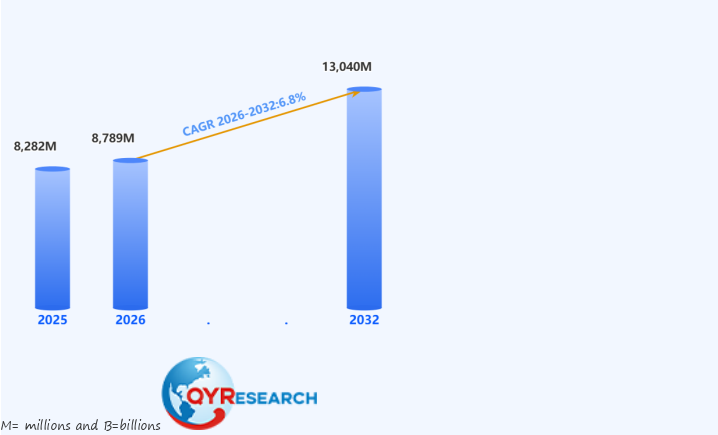
\includegraphics[width=0.8\textwidth]{figures/nfc_market.png}
	\caption{全球 NFC 控制芯片市场规模及预测}
	\label{fig:nfc_market}
\end{figure}

\textbf{2. 技术架构与实现路径}
\begin{itemize}
	\item 通过手机NFC场强感应取电，无需内置电池，确保产品轻薄化（厚度 $<0.8$ 毫米）和免维护。
	\item 签名生成时间控制在50毫秒以内，验证在30毫秒以内，确保总响应时间 $<0.5$ 秒。
	\item 私钥存储于安全芯片受保护存储区，公钥通过安全通道上传至权限管理平台，完成身份绑定。
\end{itemize}

\textbf{3. 商业模式与收入结构} \\
本阶段以\textbf{硬件销售为主导，辅以咨询服务}。NFC贴片参照高安全场景的 DESFire 级产品，毛利率设定在30\%-40\%。同时，为大型企业提供高利润的后量子迁移规划咨询服务。

% 预留图片位置：PQC市场规模图
\begin{figure}[htbp]
	\centering
	% 请将图片命名为 pqc_market.png 并放入 images 文件夹下，然后取消下一行的注释
	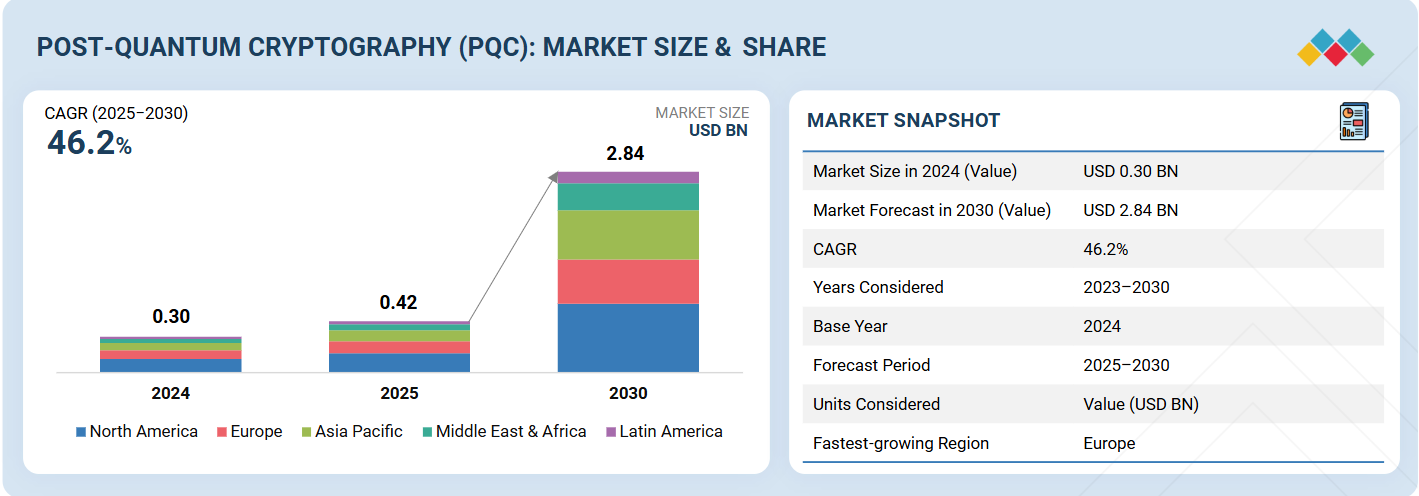
\includegraphics[width=0.85\textwidth]{figures/pqc_market.png}
	\caption{全球后量子密码 (PQC) 市场规模预测}
	\label{fig:pqc_market}
\end{figure}

\subsection{Phase 2：门禁系统升级期（18-36个月）}

\textbf{1. 产品定位与核心价值} \\
核心任务是从单一贴片向\textbf{“贴片+门锁+平台”}一体化系统升级。推出支持PQC算法的终端读卡器/门锁，与PQC贴片配合形成端到端安全链路。根据 Global Growth Insights 数据，基于云的访问控制已占新项目的近33\%。

\textbf{2. 技术架构与实现路径} \\
采用NIST标准：ML-KEM 用于密钥封装，ML-DSA 用于数字签名。系统架构采用\textbf{双栈兼容模式}：同时支持 ML-DSA 和 ECC 签名验证，客户可分批次完成升级，大幅降低迁移门槛。

% 预留图片位置：智能门锁规模图
\begin{figure}[htbp]
	\centering
	% 请将图片命名为 lock_market.png 并放入 images 文件夹下，然后取消下一行的注释
	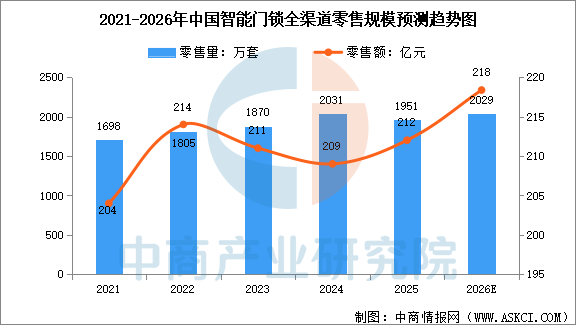
\includegraphics[width=0.8\textwidth]{figures/lock_market.png}
	\caption{2021-2026年中国智能门锁全渠道零售规模预测}
	\label{fig:lock_market}
\end{figure}

\textbf{3. 商业模式与收入结构} \\
从单一硬件向\textbf{“硬件+平台订阅”}转型。平台按节点数收取年费（约 50-80元/年/节点），包含云平台使用费、密钥管理与安全运维。

\subsection{Phase 3：后量子安全平台生态期（36-60个月）}

\textbf{1. 产品定位与核心价值} \\
将安全能力从单一门禁延伸至行业级\textbf{后量子安全中台}。随着NIST标准的确立，PQC生态系统正向云平台、OT设备制造等全领域扩展。

\textbf{2. 平台发布与生态构建} \\
推出“后量子安全服务平台”，提供：密钥全生命周期管理、设备身份认证与权限控制、安全态势感知、安全审计与溯源四大核心模块。

\textbf{3. 商业模式与盈利升级} \\
升级为\textbf{“平台SaaS + 生态分成”}双轮驱动。随着物联网设备的指数级增长，订阅收入规模效应显现。单卡成本将因规模效应及封装工艺优化，进一步降至 5 元以内。

\subsection{三阶段发展路径总结}

\begin{table}[htbp]
	\centering
	\caption{项目三阶段发展路径核心指标总结}
	\label{tab:three_phases_summary}
	\renewcommand{\arraystretch}{1.4}
	\small
	\begin{tabular}{p{1.5cm}p{3.5cm}p{4cm}p{4.5cm}}
		\toprule
		\textbf{维度} & \textbf{Phase 1: 贴片切入期} & \textbf{Phase 2: 系统升级期} & \textbf{Phase 3: 平台生态期} \\
		\midrule
		\textbf{时间} & 0-18个月 & 18-36个月 & 36-60个月 \\
		\textbf{核心产品} & NFC贴片 (ECC/混合) & PQC贴片+终端+云平台 & 行业级后量子安全平台 \\
		\textbf{技术架构} & ECC签名, NFC通信 & ML-KEM + ML-DSA双栈 & 平台化PQC能力, 开放API \\
		\textbf{收入模式} & 硬件销售 + 迁移咨询 & 硬件销售 + \textbf{平台订阅} & \textbf{平台SaaS} + 生态分成 \\
		\textbf{关键指标} & 完成国密认证, 2-3个标杆 & 贴片成本10-15元, ARR达350万 & 单片成本<5元, 净利率>40\% \\
		\textbf{战略目标} & 建立客户基础, 储备需求 & 释放PQC技术价值, 锁定客户 & 构建行业标准, 打造生态 \\
		\bottomrule
	\end{tabular}
\end{table}

\section{财务预测（5年）}

结合PQC市场和门禁市场的增长趋势，编制五年收入预测如下（单位：万元）：

\begin{table}[htbp]
	\centering
	\caption{5年期财务收入结构预测 (万元)}
	\label{tab:financial_forecast_5y}
	\renewcommand{\arraystretch}{1.4}
	\begin{tabular}{cp{2.5cm}cp{3cm}cc}
		\toprule
		\textbf{年度} & \textbf{硬件销售收入} & \textbf{SaaS订阅收入} & \textbf{咨询与服务收入} & \textbf{总收入} & \textbf{同比增速} \\
		\midrule
		\textbf{Y1} & 80 & — & 120 & \textbf{200} & — \\
		\textbf{Y2} & 680 & 8 & 180 & \textbf{868} & \textbf{334\%} \\
		\textbf{Y3} & 2,500 & 80 & 100 & \textbf{2,680} & \textbf{209\%} \\
		\textbf{Y4} & 4,800 & 450 & 50 & \textbf{5,300} & \textbf{98\%} \\
		\textbf{Y5} & 7,500 & 1,200 & 20 & \textbf{8,720} & \textbf{65\%} \\
		\bottomrule
	\end{tabular}
\end{table}

\textbf{关键财务指标分析：}
\begin{enumerate}
	\item \textbf{LTV/CAC 极佳}：以中型企业客户为例，获客成本(CAC)约1.2-1.5万元。按平均订阅周期4年计算，客户生命周期价值(LTV)约7.2万元，\textbf{LTV/CAC比值达 5.0-5.5}，客户单位经济模型极其健康。
	\item \textbf{ARR 快速增长}：经常性收入(ARR)从Y3的80万元增至Y5的1,200万元，三年增长15倍，平台化转型成效显著。
	\item \textbf{盈亏平衡点}：综合盈亏平衡点出现在 \textbf{Y3末至Y4初}。
	\item \textbf{毛利率趋势}：硬件毛利率从25\%提升至56\%，平台SaaS稳定在75\%-80\%，Y5净利润率可达\textbf{40.0\%}。
\end{enumerate}